% Created by tikzDevice version 0.9 on 2015-12-20 19:42:59
% !TEX encoding = UTF-8 Unicode
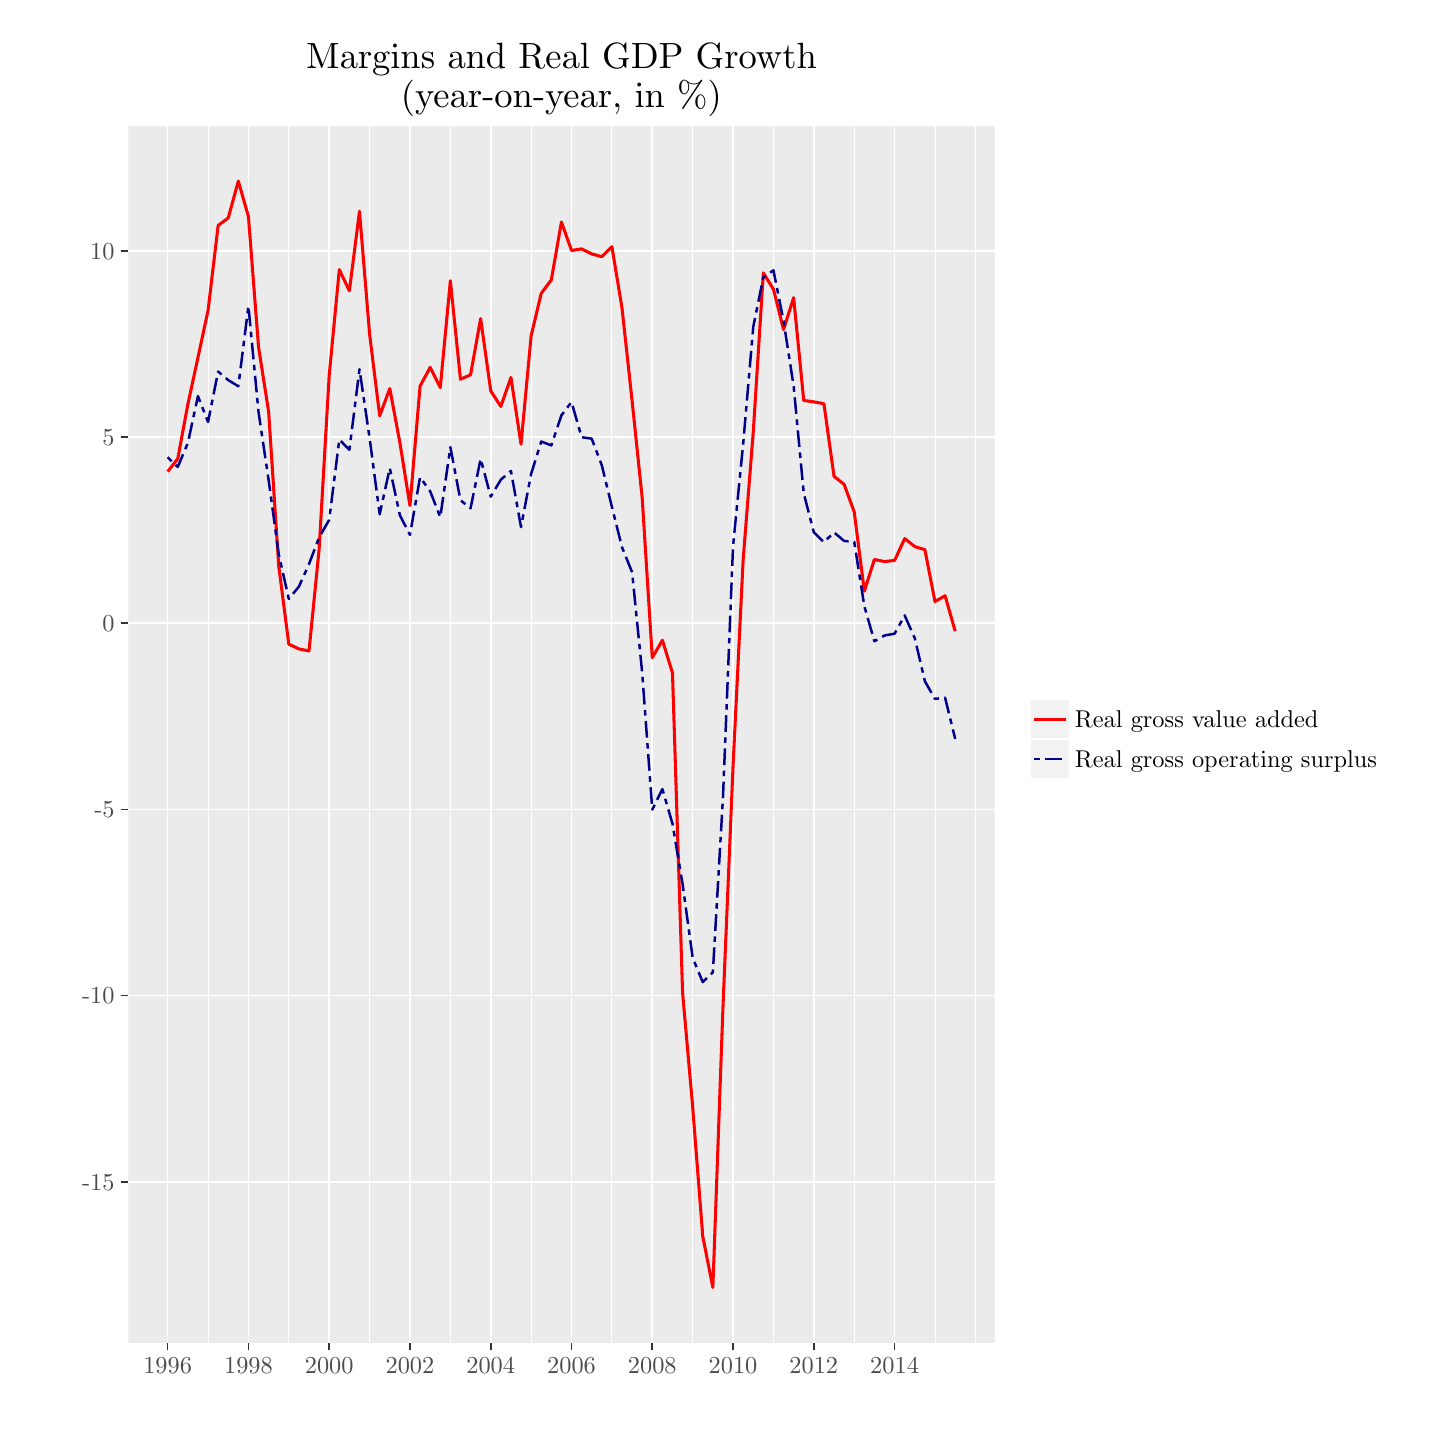
\begin{tikzpicture}[x=1pt,y=1pt]
\definecolor{fillColor}{RGB}{255,255,255}
\path[use as bounding box,fill=fillColor,fill opacity=0.00] (0,0) rectangle (505.89,505.89);
\begin{scope}
\path[clip] (  0.00,  0.00) rectangle (505.89,505.89);
\definecolor{drawColor}{RGB}{255,255,255}
\definecolor{fillColor}{RGB}{255,255,255}

\path[draw=drawColor,line width= 0.6pt,line join=round,line cap=round,fill=fillColor] (  0.00,  0.00) rectangle (505.89,505.89);
\end{scope}
\begin{scope}
\path[clip] ( 36.36, 30.69) rectangle (349.38,470.44);
\definecolor{fillColor}{gray}{0.92}

\path[fill=fillColor] ( 36.36, 30.69) rectangle (349.38,470.44);
\definecolor{drawColor}{RGB}{255,255,255}

\path[draw=drawColor,line width= 0.3pt,line join=round] ( 65.18, 30.69) --
	( 65.18,470.44);

\path[draw=drawColor,line width= 0.3pt,line join=round] ( 94.36, 30.69) --
	( 94.36,470.44);

\path[draw=drawColor,line width= 0.3pt,line join=round] (123.55, 30.69) --
	(123.55,470.44);

\path[draw=drawColor,line width= 0.3pt,line join=round] (152.74, 30.69) --
	(152.74,470.44);

\path[draw=drawColor,line width= 0.3pt,line join=round] (181.92, 30.69) --
	(181.92,470.44);

\path[draw=drawColor,line width= 0.3pt,line join=round] (211.11, 30.69) --
	(211.11,470.44);

\path[draw=drawColor,line width= 0.3pt,line join=round] (240.30, 30.69) --
	(240.30,470.44);

\path[draw=drawColor,line width= 0.3pt,line join=round] (269.48, 30.69) --
	(269.48,470.44);

\path[draw=drawColor,line width= 0.3pt,line join=round] (298.67, 30.69) --
	(298.67,470.44);

\path[draw=drawColor,line width= 0.3pt,line join=round] (327.85, 30.69) --
	(327.85,470.44);

\path[draw=drawColor,line width= 0.3pt,line join=round] (342.45, 30.69) --
	(342.45,470.44);

\path[draw=drawColor,line width= 0.6pt,line join=round] ( 36.36, 88.85) --
	(349.38, 88.85);

\path[draw=drawColor,line width= 0.6pt,line join=round] ( 36.36,156.13) --
	(349.38,156.13);

\path[draw=drawColor,line width= 0.6pt,line join=round] ( 36.36,223.41) --
	(349.38,223.41);

\path[draw=drawColor,line width= 0.6pt,line join=round] ( 36.36,290.70) --
	(349.38,290.70);

\path[draw=drawColor,line width= 0.6pt,line join=round] ( 36.36,357.98) --
	(349.38,357.98);

\path[draw=drawColor,line width= 0.6pt,line join=round] ( 36.36,425.26) --
	(349.38,425.26);

\path[draw=drawColor,line width= 0.6pt,line join=round] ( 50.58, 30.69) --
	( 50.58,470.44);

\path[draw=drawColor,line width= 0.6pt,line join=round] ( 79.77, 30.69) --
	( 79.77,470.44);

\path[draw=drawColor,line width= 0.6pt,line join=round] (108.96, 30.69) --
	(108.96,470.44);

\path[draw=drawColor,line width= 0.6pt,line join=round] (138.14, 30.69) --
	(138.14,470.44);

\path[draw=drawColor,line width= 0.6pt,line join=round] (167.33, 30.69) --
	(167.33,470.44);

\path[draw=drawColor,line width= 0.6pt,line join=round] (196.52, 30.69) --
	(196.52,470.44);

\path[draw=drawColor,line width= 0.6pt,line join=round] (225.70, 30.69) --
	(225.70,470.44);

\path[draw=drawColor,line width= 0.6pt,line join=round] (254.89, 30.69) --
	(254.89,470.44);

\path[draw=drawColor,line width= 0.6pt,line join=round] (284.07, 30.69) --
	(284.07,470.44);

\path[draw=drawColor,line width= 0.6pt,line join=round] (313.26, 30.69) --
	(313.26,470.44);
\definecolor{drawColor}{RGB}{255,0,0}

\path[draw=drawColor,line width= 1.1pt,line join=round] ( 50.58,345.47) --
	( 54.23,350.11) --
	( 57.88,369.78) --
	( 61.53,386.69) --
	( 65.18,403.68) --
	( 68.83,434.41) --
	( 72.47,437.13) --
	( 76.12,450.45) --
	( 79.77,437.63) --
	( 83.42,390.51) --
	( 87.07,367.10) --
	( 90.72,311.35) --
	( 94.36,283.11) --
	( 98.01,281.41) --
	(101.66,280.68) --
	(105.31,317.40) --
	(108.96,380.31) --
	(112.61,418.46) --
	(116.25,410.78) --
	(119.90,439.55) --
	(123.55,395.16) --
	(127.20,365.64) --
	(130.85,375.49) --
	(134.50,355.89) --
	(138.14,333.18) --
	(141.79,376.37) --
	(145.44,383.14) --
	(149.09,375.85) --
	(152.74,414.45) --
	(156.38,378.85) --
	(160.03,380.45) --
	(163.68,400.77) --
	(167.33,374.64) --
	(170.98,369.01) --
	(174.63,379.50) --
	(178.27,355.35) --
	(181.92,394.54) --
	(185.57,409.86) --
	(189.22,414.75) --
	(192.87,435.67) --
	(196.52,425.37) --
	(200.16,425.95) --
	(203.81,424.13) --
	(207.46,423.13) --
	(211.11,426.75) --
	(214.76,404.57) --
	(218.41,371.01) --
	(222.05,335.98) --
	(225.70,278.23) --
	(229.35,284.54) --
	(233.00,272.74) --
	(236.65,157.16) --
	(240.30,115.86) --
	(243.94, 69.13) --
	(247.59, 50.68) --
	(251.24,151.98) --
	(254.89,239.20) --
	(258.54,313.70) --
	(262.19,359.83) --
	(265.83,417.28) --
	(269.48,411.38) --
	(273.13,396.79) --
	(276.78,408.33) --
	(280.43,371.18) --
	(284.07,370.67) --
	(287.72,370.00) --
	(291.37,343.75) --
	(295.02,340.85) --
	(298.67,330.90) --
	(302.32,302.26) --
	(305.96,313.72) --
	(309.61,312.96) --
	(313.26,313.38) --
	(316.91,321.27) --
	(320.56,318.38) --
	(324.21,317.25) --
	(327.85,298.53) --
	(331.50,300.61) --
	(335.15,287.81);
\definecolor{drawColor}{RGB}{0,0,139}

\path[draw=drawColor,line width= 0.9pt,dash pattern=on 2pt off 2pt on 6pt off 2pt ,line join=round] ( 50.58,350.63) --
	( 54.23,347.16) --
	( 57.88,355.80) --
	( 61.53,372.74) --
	( 65.18,363.39) --
	( 68.83,381.62) --
	( 72.47,378.54) --
	( 76.12,376.30) --
	( 79.77,405.31) --
	( 83.42,366.96) --
	( 87.07,342.39) --
	( 90.72,315.58) --
	( 94.36,299.46) --
	( 98.01,303.92) --
	(101.66,312.07) --
	(105.31,321.68) --
	(108.96,328.05) --
	(112.61,357.09) --
	(116.25,353.32) --
	(119.90,382.45) --
	(123.55,357.63) --
	(127.20,330.05) --
	(130.85,346.73) --
	(134.50,329.68) --
	(138.14,322.61) --
	(141.79,343.44) --
	(145.44,338.37) --
	(149.09,329.00) --
	(152.74,354.32) --
	(156.38,335.14) --
	(160.03,332.20) --
	(163.68,350.08) --
	(167.33,336.43) --
	(170.98,342.56) --
	(174.63,345.70) --
	(178.27,325.42) --
	(181.92,344.65) --
	(185.57,356.34) --
	(189.22,354.94) --
	(192.87,365.81) --
	(196.52,370.62) --
	(200.16,357.90) --
	(203.81,357.36) --
	(207.46,347.77) --
	(211.11,332.72) --
	(214.76,318.14) --
	(218.41,309.11) --
	(222.05,272.78) --
	(225.70,223.35) --
	(229.35,230.75) --
	(233.00,218.24) --
	(236.65,196.38) --
	(240.30,169.76) --
	(243.94,160.99) --
	(247.59,164.56) --
	(251.24,227.66) --
	(254.89,318.70) --
	(258.54,355.47) --
	(262.19,397.81) --
	(265.83,415.70) --
	(269.48,418.21) --
	(273.13,399.90) --
	(276.78,376.39) --
	(280.43,337.62) --
	(284.07,323.54) --
	(287.72,319.97) --
	(291.37,323.51) --
	(295.02,320.41) --
	(298.67,320.11) --
	(302.32,296.85) --
	(305.96,284.17) --
	(309.61,286.25) --
	(313.26,286.91) --
	(316.91,293.49) --
	(320.56,285.25) --
	(324.21,269.71) --
	(327.85,263.33) --
	(331.50,263.78) --
	(335.15,248.90);
\end{scope}
\begin{scope}
\path[clip] (  0.00,  0.00) rectangle (505.89,505.89);
\definecolor{drawColor}{gray}{0.30}

\node[text=drawColor,anchor=base east,inner sep=0pt, outer sep=0pt, scale=  0.88] at ( 31.41, 85.82) {-15};

\node[text=drawColor,anchor=base east,inner sep=0pt, outer sep=0pt, scale=  0.88] at ( 31.41,153.10) {-10};

\node[text=drawColor,anchor=base east,inner sep=0pt, outer sep=0pt, scale=  0.88] at ( 31.41,220.38) {-5};

\node[text=drawColor,anchor=base east,inner sep=0pt, outer sep=0pt, scale=  0.88] at ( 31.41,287.67) {0};

\node[text=drawColor,anchor=base east,inner sep=0pt, outer sep=0pt, scale=  0.88] at ( 31.41,354.95) {5};

\node[text=drawColor,anchor=base east,inner sep=0pt, outer sep=0pt, scale=  0.88] at ( 31.41,422.23) {10};
\end{scope}
\begin{scope}
\path[clip] (  0.00,  0.00) rectangle (505.89,505.89);
\definecolor{drawColor}{gray}{0.20}

\path[draw=drawColor,line width= 0.6pt,line join=round] ( 33.61, 88.85) --
	( 36.36, 88.85);

\path[draw=drawColor,line width= 0.6pt,line join=round] ( 33.61,156.13) --
	( 36.36,156.13);

\path[draw=drawColor,line width= 0.6pt,line join=round] ( 33.61,223.41) --
	( 36.36,223.41);

\path[draw=drawColor,line width= 0.6pt,line join=round] ( 33.61,290.70) --
	( 36.36,290.70);

\path[draw=drawColor,line width= 0.6pt,line join=round] ( 33.61,357.98) --
	( 36.36,357.98);

\path[draw=drawColor,line width= 0.6pt,line join=round] ( 33.61,425.26) --
	( 36.36,425.26);
\end{scope}
\begin{scope}
\path[clip] (  0.00,  0.00) rectangle (505.89,505.89);
\definecolor{drawColor}{gray}{0.20}

\path[draw=drawColor,line width= 0.6pt,line join=round] ( 50.58, 27.94) --
	( 50.58, 30.69);

\path[draw=drawColor,line width= 0.6pt,line join=round] ( 79.77, 27.94) --
	( 79.77, 30.69);

\path[draw=drawColor,line width= 0.6pt,line join=round] (108.96, 27.94) --
	(108.96, 30.69);

\path[draw=drawColor,line width= 0.6pt,line join=round] (138.14, 27.94) --
	(138.14, 30.69);

\path[draw=drawColor,line width= 0.6pt,line join=round] (167.33, 27.94) --
	(167.33, 30.69);

\path[draw=drawColor,line width= 0.6pt,line join=round] (196.52, 27.94) --
	(196.52, 30.69);

\path[draw=drawColor,line width= 0.6pt,line join=round] (225.70, 27.94) --
	(225.70, 30.69);

\path[draw=drawColor,line width= 0.6pt,line join=round] (254.89, 27.94) --
	(254.89, 30.69);

\path[draw=drawColor,line width= 0.6pt,line join=round] (284.07, 27.94) --
	(284.07, 30.69);

\path[draw=drawColor,line width= 0.6pt,line join=round] (313.26, 27.94) --
	(313.26, 30.69);
\end{scope}
\begin{scope}
\path[clip] (  0.00,  0.00) rectangle (505.89,505.89);
\definecolor{drawColor}{gray}{0.30}

\node[text=drawColor,anchor=base,inner sep=0pt, outer sep=0pt, scale=  0.88] at ( 50.58, 19.68) {1996};

\node[text=drawColor,anchor=base,inner sep=0pt, outer sep=0pt, scale=  0.88] at ( 79.77, 19.68) {1998};

\node[text=drawColor,anchor=base,inner sep=0pt, outer sep=0pt, scale=  0.88] at (108.96, 19.68) {2000};

\node[text=drawColor,anchor=base,inner sep=0pt, outer sep=0pt, scale=  0.88] at (138.14, 19.68) {2002};

\node[text=drawColor,anchor=base,inner sep=0pt, outer sep=0pt, scale=  0.88] at (167.33, 19.68) {2004};

\node[text=drawColor,anchor=base,inner sep=0pt, outer sep=0pt, scale=  0.88] at (196.52, 19.68) {2006};

\node[text=drawColor,anchor=base,inner sep=0pt, outer sep=0pt, scale=  0.88] at (225.70, 19.68) {2008};

\node[text=drawColor,anchor=base,inner sep=0pt, outer sep=0pt, scale=  0.88] at (254.89, 19.68) {2010};

\node[text=drawColor,anchor=base,inner sep=0pt, outer sep=0pt, scale=  0.88] at (284.07, 19.68) {2012};

\node[text=drawColor,anchor=base,inner sep=0pt, outer sep=0pt, scale=  0.88] at (313.26, 19.68) {2014};
\end{scope}
\begin{scope}
\path[clip] (  0.00,  0.00) rectangle (505.89,505.89);
\definecolor{fillColor}{RGB}{255,255,255}

\path[fill=fillColor] (357.91,230.04) rectangle (491.85,271.09);
\end{scope}
\begin{scope}
\path[clip] (  0.00,  0.00) rectangle (505.89,505.89);
\definecolor{drawColor}{RGB}{255,255,255}
\definecolor{fillColor}{gray}{0.95}

\path[draw=drawColor,line width= 0.6pt,line join=round,line cap=round,fill=fillColor] (362.18,248.76) rectangle (376.64,263.21);
\end{scope}
\begin{scope}
\path[clip] (  0.00,  0.00) rectangle (505.89,505.89);
\definecolor{drawColor}{RGB}{255,0,0}

\path[draw=drawColor,line width= 1.1pt,line join=round] (363.63,255.99) -- (375.19,255.99);
\end{scope}
\begin{scope}
\path[clip] (  0.00,  0.00) rectangle (505.89,505.89);
\definecolor{drawColor}{RGB}{255,255,255}
\definecolor{fillColor}{gray}{0.95}

\path[draw=drawColor,line width= 0.6pt,line join=round,line cap=round,fill=fillColor] (362.18,234.30) rectangle (376.64,248.76);
\end{scope}
\begin{scope}
\path[clip] (  0.00,  0.00) rectangle (505.89,505.89);
\definecolor{drawColor}{RGB}{0,0,139}

\path[draw=drawColor,line width= 0.9pt,dash pattern=on 2pt off 2pt on 6pt off 2pt ,line join=round] (363.63,241.53) -- (375.19,241.53);
\end{scope}
\begin{scope}
\path[clip] (  0.00,  0.00) rectangle (505.89,505.89);
\definecolor{drawColor}{RGB}{0,0,0}

\node[text=drawColor,anchor=base west,inner sep=0pt, outer sep=0pt, scale=  0.88] at (378.44,252.95) {Real gross value added};
\end{scope}
\begin{scope}
\path[clip] (  0.00,  0.00) rectangle (505.89,505.89);
\definecolor{drawColor}{RGB}{0,0,0}

\node[text=drawColor,anchor=base west,inner sep=0pt, outer sep=0pt, scale=  0.88] at (378.44,238.50) {Real gross operating surplus};
\end{scope}
\begin{scope}
\path[clip] (  0.00,  0.00) rectangle (505.89,505.89);
\definecolor{drawColor}{RGB}{0,0,0}

\node[text=drawColor,anchor=base,inner sep=0pt, outer sep=0pt, scale=  1.32] at (192.87,491.30) {Margins and Real GDP Growth};

\node[text=drawColor,anchor=base,inner sep=0pt, outer sep=0pt, scale=  1.32] at (192.87,477.04) {(year-on-year, in {\%})};
\end{scope}
\end{tikzpicture}
